%%%%%%%%%%%%%%%%%%%%%%%%%%%%%%%%%%%%%%%%%%%%%%%%%%%%%%%%%%%%%%%%%%%%%%%%
%%%  THIS TEX FILE IS TO GENERATE PDF FILE FOR 
%%% 
%%%  COPYRIGHT (C) JIMMY LIN, 2013, UT AUSTIN
%%%%%%%%%%%%%%%%%%%%%%%%%%%%%%%%%%%%%%%%%%%%%%%%%%%%%%%%%%%%%%%%%%%%%%%%
\documentclass[11pt,a4paper]{article}
%%%%%%%%%%%%%%%%%%%%%%%%%%%%%%%%%%%%%%%%%%%%%%%%%%%%%%%%%%%%%%%%%%%%%%%%
%%%  PACKAGES USED IN THIS TEX SOURCE FILE
%%%%%%%%%%%%%%%%%%%%%%%%%%%%%%%%%%%%%%%%%%%%%%%%%%%%%%%%%%%%%%%%%%%%%%%%
\usepackage{geometry,amsthm,amsmath,graphicx,amssymb,fancyheadings}
\usepackage[]{mcode}
\usepackage[colorlinks,
            linkcolor=blue,
            anchorcolor=red,
            citecolor=green
            ]{hyperref}
% for my mac
\IfFileExists{/Users/JimmyLin/.latex/UTA_CS/JS.sty}{ 
    \usepackage{/Users/JimmyLin/.latex/UTA_CS/JS}
    \usepackage{/Users/JimmyLin/.latex/UTA_CS/JSASGN}
}{} 
% for UT's linux machine
\IfFileExists{/u/jimmylin/workspace/Configs/latex/UTA_CS/JS.sty}{
    \usepackage{/u/jimmylin/.latex/UTA_CS/JS} 
    \usepackage{/u/jimmylin/.latex/UTA_CS/JSASGN}
}{} 
%%%%%%%%%%%%%%%%%%%%%%%%%%%%%%%%%%%%%%%%%%%%%%%%%%%%%%%%%%%%%%%%%%%%%%%%
%%% MACROS CONTAINING THE FILE INFORMATION
%%%%%%%%%%%%%%%%%%%%%%%%%%%%%%%%%%%%%%%%%%%%%%%%%%%%%%%%%%%%%%%%%%%%%%%%
\renewcommand{\COURSE}{EE381V Large Scale Optimization}
\renewcommand{\LECTURER}{Sujay Sanghavi}
\renewcommand{\SECTION}{17350}
\renewcommand{\TASK}{Problem Set 1}
\renewcommand{\RELEASEDATE}{September 15, 2014}
\renewcommand{\DUEDATE}{September 23, 2014}
\renewcommand{\TIMECONSUME}{13 hours}
%%%%%%%%%%%%%%%%%%%%%%%%%%%%%%%%%%%%%%%%%%%%%%%%%%%%%%%%%%%%%%%%%%%%%%%%
%%% DOCUMENTATION STARTS FROM HERE 
%%%%%%%%%%%%%%%%%%%%%%%%%%%%%%%%%%%%%%%%%%%%%%%%%%%%%%%%%%%%%%%%%%%%%%%%

\begin{document}
%%%%%%%%%%%%%%%%%%%%%%%%%%%%%%%%%%%%%%%%%%%%%%%%%%%%%%%%%%%%%%%%%%%%%%%%
%% TITLE PAGE
%%%%%%%%%%%%%%%%%%%%%%%%%%%%%%%%%%%%%%%%%%%%%%%%%%%%%%%%%%%%%%%%%%%%%%%%
\begin{titlepage}
    \maketitle
\end{titlepage}
%%%%%%%%%%%%%%%%%%%%%%%%%%%%%%%%%%%%%%%%%%%%%%%%%%%%%%%%%%%%%%%%%%%%%%%%
%% CONTENT PAGE: TABLEOFCONTENTS, LISTOFTABLES, LIST OF FIGURES
%%%%%%%%%%%%%%%%%%%%%%%%%%%%%%%%%%%%%%%%%%%%%%%%%%%%%%%%%%%%%%%%%%%%%%%%
\renewcommand{\contentsname}{Table of Contents}
\begin{center} 
    \tableofcontents 
    %\listoftables 
    \listoffigures
\end{center}
\newpage
%%%%%%%%%%%%%%%%%%%%%%%%%%%%%%%%%%%%%%%%%%%%%%%%%%%%%%%%%%%%%%%%%%%%%%%%
%%% GENERAL DOCUMENTATION BEGINS 
%%%%%%%%%%%%%%%%%%%%%%%%%%%%%%%%%%%%%%%%%%%%%%%%%%%%%%%%%%%%%%%%%%%%%%%%

\part{Matlab and Computational Assignment}
\section{Gradient Descent on three matrices}
Command to get executed: 
\begin{verbatim}
   >> gd_run_script()
\end{verbatim}
\subsection{$X1$, $b1$}
\begin{itemize}
    \item Range of $\gamma$ that leads to convergence: $(0,2)$
    \item Range of $\gamma$ that leads to divergence: $(2,+\infty)$
    \item Explanation: if $\gamma = 2$, the program indicates that 
        $$ \forall k,\ f(x^{k+1}) = f(x^{k})$$ 
        Since the above equation is constantly true (independent of the
        minima), we can conclude that gradient descent with $\gamma = 2$ goes 
        to the opposite side of that quadratic curve. Intuitively, the program 
        will diverge if we set larger ($\gamma>2$) and converge if we set smaller
        ($\gamma<2$).   
    \item Two illustrative examples: $\gamma = 0.5$ and $\gamma = 3.0$
        \begin{figure}[h]
            \centering
            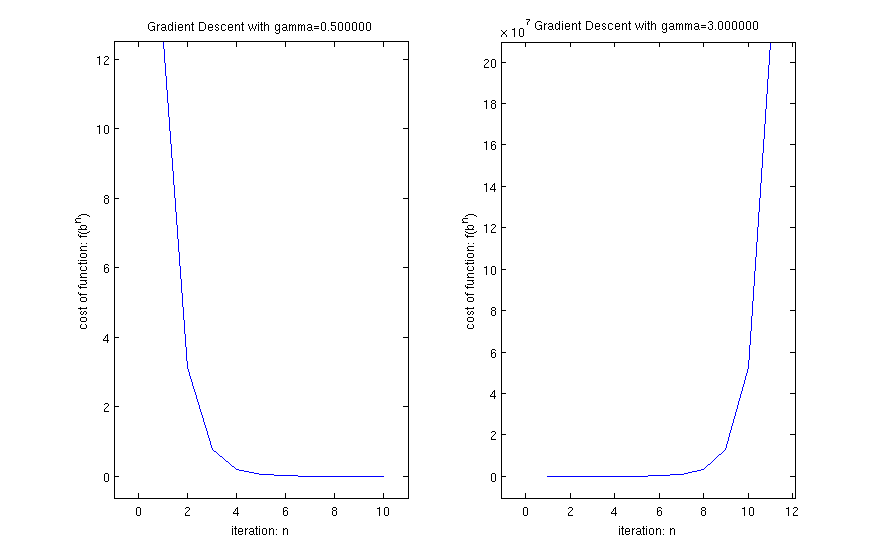
\includegraphics[width=6in,height=3in]{../ps1_matlab/1.png}
            \caption{Illustration for gradient descent on $X1$, staring with
                $b1$ by $\gamma = 0.5$ and $3.0$}
        \end{figure}
\end{itemize}

\newpage
\subsection{$X2$, $b2$}
\begin{itemize}
    \item Range of $\gamma$ that leads to convergence: $(0,2)$
    \item Range of $\gamma$ that leads to divergence: $(2,+\infty)$
    \item Explanation: if $\gamma = 2$, the program indicates that 
        $$ \forall k,\ f(x^{k+1}) = f(x^{k})$$ 
        Since the above equation is constantly true (independent of the
        minima), we can conclude that gradient descent with $\gamma = 2$ goes 
        to the opposite side of that quadratic curve. Intuitively, the program 
        will diverge if we set larger ($\gamma>2$) and converge if we set smaller
        ($\gamma<2$).
    \item Two illustrative
        examples: $\gamma = 1.5$ and $\gamma = 3.0$
        \begin{figure}[h]
            \centering
            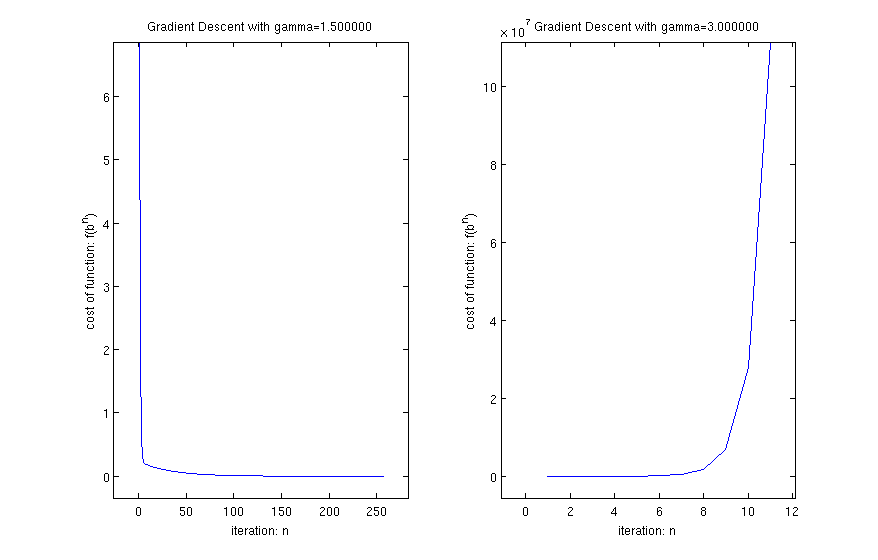
\includegraphics[width=6in,height=3in]{../ps1_matlab/2.png}
            \caption{Illustration for gradient descent on $X2$, starting with
                $b2$ by $\gamma = 1.5$ and $3.0$}
        \end{figure}
\end{itemize}

\newpage
\subsection{$X3$, $b3$}
\begin{itemize}
    \item Range of $\gamma$ that leads to convergence: $(0,0.02)$
    \item Range of $\gamma$ that leads to divergence: $(0.02,+\infty)$
    \item Explanation: if $\gamma = 0.02$, the program indicates that 
        $$ \forall k,\ f(x^{k+1}) = f(x^{k})$$ 
        Since the above equation is constantly true (independent of the
        minima), we can conclude that gradient descent with $\gamma = 0.02$ goes 
        to the opposite side of that quadratic curve. Intuitively, the program 
        will diverge if we set larger ($\gamma>0.02$) and converge if we set smaller
        ($\gamma<0.02$).
    \item Two illustrative examples: $\gamma = 0.005$ and $\gamma = 0.05$
        \begin{figure}[h]
            \centering
            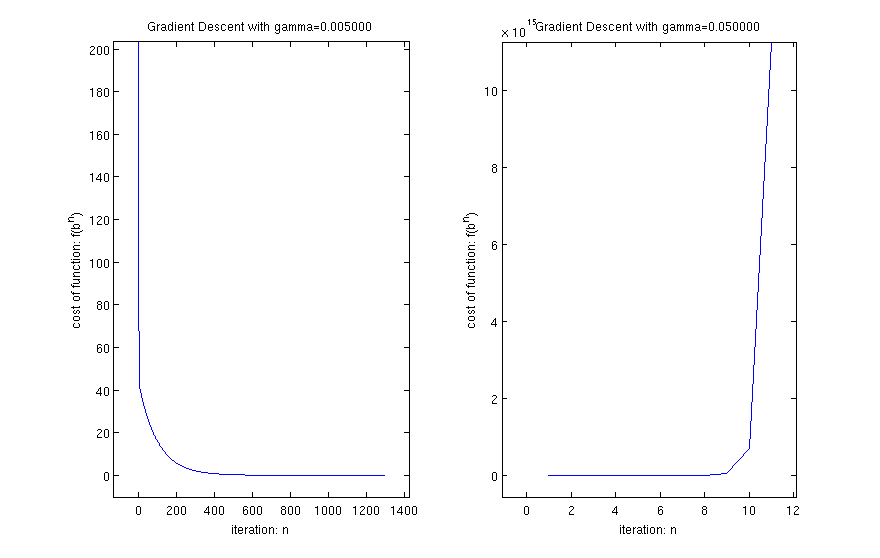
\includegraphics[width=6in,height=3in]{../ps1_matlab/3.png}
            \caption{Illustration for gradient descent on $X3$ staring with
                $b3$ by $\gamma = 0.005$ and $0.05$}
        \end{figure}
\end{itemize}

\newpage
\section{$\gamma = 1$ for the second matrix}
Command to get executed: 
\begin{verbatim}
   >> gamma = 1;
   >> [b2_opt, iters, all_costs] = gd (X2, b2, gamma);
\end{verbatim}
{\bf Plotting}: figure for $\gamma = 1$
\begin{figure}[h]
            \centering
            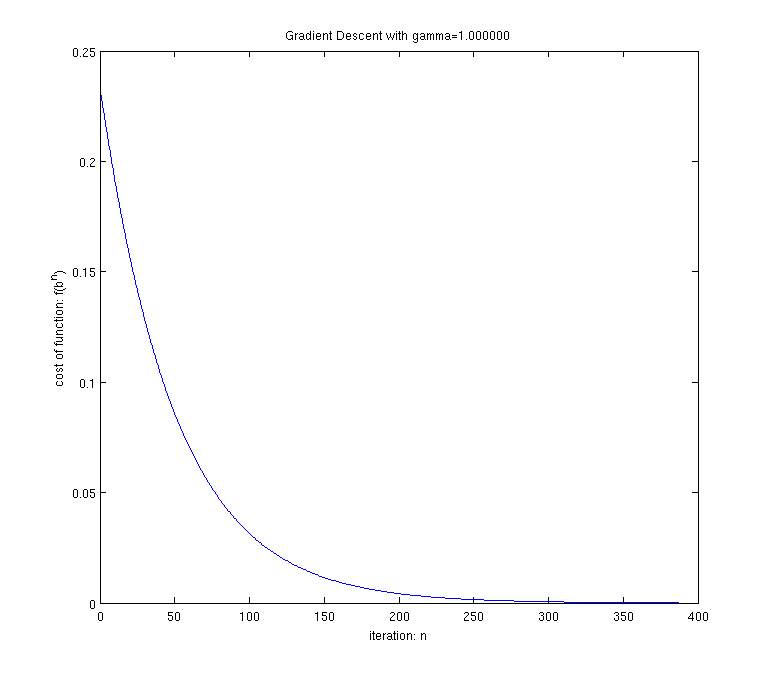
\includegraphics[width=4in,height=3in]{../ps1_matlab/2_gamma1.png}
            \caption{Plotting figure for gradient descent with $\gamma = 1$ on
            the second matrix}
\end{figure}

\noindent
{\bf Explanation}: 
Through the smooth plotted curve, we guess that the gradient
descent method got linear convergence when $\gamma=1$ on $X_2$. Hence, we trace
convergence rate conv\_rate $ = f(x^{k}) / f(x^{k-1})$ as follows:
\begin{verbatim}
Iter: 2, Cost: 2.254428e-01, Conv_Rate: 0.980100
Iter: 3, Cost: 2.209565e-01, Conv_Rate: 0.980100
Iter: 4, Cost: 2.165594e-01, Conv_Rate: 0.980100
Iter: 5, Cost: 2.122499e-01, Conv_Rate: 0.980100
Iter: 6, Cost: 2.080261e-01, Conv_Rate: 0.980100
Iter: 7, Cost: 2.038864e-01, Conv_Rate: 0.980100
...
...
Iter: 381, Cost: 1.107934e-04, Conv_Rate: 0.980100
Iter: 382, Cost: 1.085886e-04, Conv_Rate: 0.980100
Iter: 383, Cost: 1.064277e-04, Conv_Rate: 0.980100
Iter: 384, Cost: 1.043098e-04, Conv_Rate: 0.980100
Iter: 385, Cost: 1.022340e-04, Conv_Rate: 0.980100
Iter: 386, Cost: 1.001996e-04, Conv_Rate: 0.980100
Iter: 387, Cost: 9.820558e-05, Conv_Rate: 0.980100
Converged to zeros!
\end{verbatim}
In terms of above dumps and the fact that $f(x^{*}) = 0$, we can conclude that when $\gamma = 1$        
$$
f(x^{k+1}) - f(x^{*}) = 0.9801 \cdot \big( f(x^{k}) - f(x^{*}) \big)
$$
which supports our previous guess that
$$ 
\text{Gradient Descent with }
\gamma = 1
\text{ on second matrix leads to {\bf linear convergence}. }
$$

\newpage
%%%%%%%%%%%%%%%%%%%%%%%%%%%%%%%%%%%%%%%%%%%%%%%%%%%%%%%%%%%%
%%% Written Problems
%%%%%%%%%%%%%%%%%%%%%%%%%%%%%%%%%%%%%%%%%%%%%%%%%%%%%%%%%%%%
\newpage
\part{Written Problems}
\setcounter{section}{0}
\renewcommand{\thesubsection}{(\alph{subsection})}
\section{Othorognal Subspace}
\newcommand{\Ut}{U^{\perp}}
\newcommand{\ut}{u^{\perp}}
\newcommand{\Wt}{W^{\perp}}
\newcommand{\Xt}{X^{\perp}}
\newcommand{\zerovec}{\mathbf{0}} 
\newcommand{\uvec}{\mathbf{u}}
\newcommand{\vvec}{\mathbf{v}}
\newcommand{\wvec}{\mathbf{w}}
\newcommand{\xvec}{\mathbf{x}}
\subsection{Show that if $U$ is a subspace, then so is $\Ut$}
\begin{proof}
    Since $U$ is a subspace, then we have $U$ satisfying all three properties
    shown below:
    \begin{itemize}
       \item $\zerovec \in U$ 
       \item $\forall \uvec_1, \uvec_2 \in U, \uvec_1 + \uvec_2 \in U$
       \item $\forall \uvec \in U, \alpha \in \mathbb{R}, \alpha \uvec \in U$
    \end{itemize}
    Now we show that $\Ut$ is also a subspace by indicating $\Ut$
    satisfies all three properties as above $U$ does.
    \begin{itemize}
        \item Since $\forall \uvec \in U, \langle \zerovec, \uvec \rangle = 0$
            and $\zerovec \in V$ ($\zerovec \in U \subseteq V$), then it
            turned out that $\zerovec \in \Ut$.
        \item Let $\uvec$ be arbitrary vector s.t. $\uvec \in U$, and
            $\xvec_1$, $\xvec_2$ to be distinct vector s.t. $\xvec_1 \in \Ut$
            and $\xvec_2 \in \Ut$. By definition of $\Ut$, we have 
            $\langle \xvec_1, \uvec \rangle = 0$ and 
            $\langle \xvec_2, \uvec \rangle = 0$. 
            Then it is obvious that 
            $\langle \xvec_1 + \xvec_2, \uvec \rangle = 0$. 
            That is $\xvec_1 +\xvec_2 \in \Ut$.
            Therefore, $\forall \xvec_1, \xvec_2 \in \Ut, \xvec_1+\xvec_2 \in \Ut$ was proved.
        \item Let $\xvec$ be arbitrary vector s.t. $\xvec \in \Ut$, 
            $\uvec$ be arbitrary vector s.t. $\uvec \in U$ and
            arbitrary $\alpha \in \mathbb{R}$. By definition of $\Ut$, we have 
            $\langle \xvec, \uvec \rangle = 0$. 
            Since inner product is linear operator, it is obvious that
            $\langle \alpha \xvec, \uvec \rangle = 0$. 
            That is $\alpha \xvec \in \Ut$.
            Therefore, $\forall \xvec \in \Ut, \alpha \in \mathbb{R}, \alpha
            \xvec \in \Ut$ was proved.
    \end{itemize}
    Since $\Ut$ contains $\zerovec$, and is closed under addition and scalar
    multiplication, it turned out that $\Ut$ is a subspace. 
    Therefore, the statement that if $U$ is a subspace, then so is $\Ut$ was
    proved.
\end{proof}
\subsection{Show that $(\Ut)^{\perp} = U$}
\begin{proof}[Proof. By contradiction.]
    Assume that $(\Ut)^{\perp} \not= U$ and then show the contradiction. 
    By definition of $\Ut$, we have
    $ \Ut = 
    \{\forall \vvec \in V, \langle \vvec, \uvec \rangle = 0, \forall \uvec \in U\}$
    and 
    $ (\Ut)^{\perp} = 
    \{\forall \xvec \in V, \langle \xvec, \vvec \rangle = 0, \forall \vvec \in \Ut\}$.
    Since $(\Ut)^{\perp} \not= U$, then we can say that 
    $ \exists \xvec \not \in U, \langle \xvec, \vvec \rangle = 0, \forall
     \vvec \in \Ut $. 
     That is to say, 
    $ \exists \xvec \in V\ but\ \not \in U, \langle \xvec, \vvec \rangle = 0, \forall
     \vvec \ s.t. \langle \vvec, \uvec \rangle = 0, \forall \uvec \in U$. 
     However, such $\xvec$ does not exist. Hence, we reject
     initial assumption and conclude that $(\Ut)^{\perp} = U$.
\end{proof}

\subsection{Show that if $U, W \subseteq V$ are subspaces of V, then $U
    \subseteq W \Leftrightarrow \Ut \supseteq \Wt$}
\begin{proof}[Proof of $U \subseteq W \Rightarrow \Ut \supseteq \Wt$]
    $\Ut = 
    \{\forall \vvec \in V, \langle \vvec, \uvec \rangle = 0, \forall \uvec \in U\} $
    and
    $\Wt = 
    \{\forall \vvec \in V, \langle \vvec, \wvec \rangle = 0, \forall \wvec \in W\} 
    = \{\forall \vvec \in V, \langle \vvec, \wvec \rangle = 0, \forall \wvec
        \in W\ \text{and } \langle \vvec, \uvec \rangle = 0, \forall \uvec \in U\} 
    $ (This is valid because $\forall U \subseteq W$ and then $\uvec \in W$).
    Now since membership of $\Wt$ requires one more condition, then it is obvious that 
    $\vvec \in \Wt \Rightarrow \vvec \in \Ut$, and $\vvec \in
    \Ut \not \Rightarrow \vvec \in \Wt$ hold for arbitrary $\vvec$. Therefore,
    we can conclude that $\Ut \supseteq \Wt$.
\end{proof}
\begin{proof}[Proof of $\Ut \supseteq \Wt \Rightarrow U \subseteq W $]
    By definition, we have
    $ \Ut = 
    \{\vvec \in V | \langle \vvec, \uvec \rangle = 0, \forall \uvec \in U\}$ and
    $\Wt = 
    \{\vvec \in V | \langle \vvec, \wvec \rangle = 0, \forall \wvec \in W\}$.
    Since $\Ut \supseteq \Wt$, then we have $\Ut \cap \Wt  = \Wt$. 
    Then 
    $
    \Ut \cap \Wt = \{\vvec \in V | \langle \vvec, \uvec \rangle = 0, \forall \uvec \in U
        \text{ and } \langle \vvec, \wvec \rangle = 0, \forall \wvec \in W\} 
    = \{ \vvec \in V | \langle \vvec, \xvec \rangle = 0, \forall \xvec \in W
        \cup U\} = \Wt$
    Then we have $W \cup U = W$, which naturally derives $U \subseteq W$.
\end{proof}

\newpage
\newcommand{\xtvec}{\mathbf{x}^{\perp}}
\subsection{Show that $\Xt$ makes sense, $\Xt$ is a subspace and
    $(\Xt)^{\perp} \supseteq X$}
\begin{proof}[Explanation of $\Xt$ makes sense]
    $\Xt$ also makes sense. This is because we can view all vectors in set $X$
    as bases of the minimal subspace that is superset of $X$. Therefore,
    although the $\Xt$ is defined through the set $X$, it makes sense as
    othogonal complement over the minimal subspace that contains $X$.
\end{proof}
\begin{proof}[Proof of $\Xt$ is a subspace]
    We prove $\Xt$ is a subspace by showing $\Xt$ satisfies three properties
    as $\Ut$ above does. 
    \begin{itemize}
        \item Since $\forall \xvec \in X, \langle \zerovec, \xvec \rangle = 0$
            and $\zerovec \in V$, then it turned out that $\zerovec \in \Xt$.
        \item Let $\xvec$ be arbitrary vector s.t. $\xvec \in U$, and
            $\xtvec_1$, $\xtvec_2$ to be distinct vector s.t. $\xtvec_1 \in \Xt$
            and $\xtvec_2 \in \Xt$. By definition of $\Xt$, we have 
            $\langle \xtvec_1, \xvec \rangle = 0$ and 
            $\langle \xtvec_2, \xvec \rangle = 0$. 
            Then it is obvious that 
            $\langle \xtvec_1 + \xtvec_2, \xvec \rangle = 0$. 
            That is, $\xtvec_1 +\xtvec_2 \in \Xt$.
            Therefore, $\forall \xtvec_1, \xtvec_2 \in \Xt,
            \xtvec_1+\xtvec_2 \in \Xt$ was proved. (That is, membership of
            $\Xt$ is closed under vector addition).
        \item Let $\xtvec$ be arbitrary vector s.t. $\xvec \in \Xt$, 
            $\xvec$ be arbitrary vector s.t. $\xvec \in X$ and
            arbitrary $\alpha \in \mathbb{R}$. By definition of $\Xt$, we have 
            $\langle \xtvec, \xvec \rangle = 0$. 
            Since inner product is linear operator, it is obvious that
            $\langle \alpha \xtvec, \xvec \rangle = 0$. 
            That is $\alpha \xtvec \in \Xt$.
            Therefore, $\forall \xtvec \in \Xt, \alpha \in \mathbb{R}, \alpha
            \xtvec \in \Xt$ was proved. (That is, membership of $\Xt$ is
            closed under scalar multiplication.)
    \end{itemize}
    Since we have shown that $\Xt$ satisfies all three above properties, then
    we conclude that $\Xt$ is a subspace.
\end{proof}

\begin{proof}[Proof of $(\Xt)^{\perp} \supseteq X$]
    Through the definition of $\Xt$, it is easy to derive the property for set $X$
    \begin{align}
        \forall x \in X,\ \langle x, x^{\perp} \rangle = 0,\ \forall x^{\perp}
        \in \Xt
    \end{align}
    And similarly, we can derive the property for subspace $(\Xt)^\perp$
    \begin{align}
        \forall x \in (\Xt)^\perp,\ \langle x, x^{\perp} \rangle = 0,\ \forall x^{\perp}
        \in \Xt
    \end{align}
    It is obvious that, all elements in set $X$ and subspace $(\Xt)^\perp$ are
    perpendicular to any vectors in $\Xt$. \\
    Since $X$ is a set with finite element, and $(\Xt)^\perp$ is a subspace
    with infinite elements, it is natural to derive that 
    \begin{align}
        (\Xt)^\perp \supseteq X
    \end{align}
\end{proof}

\newpage
\subsection{Show that any $v \in V$ can be written uniquely as $v = u + \ut$} 
\begin{proof}
    Assume that the representation of arbitrary vector $v \in V$ is not
    unique.
    Let $u_1$, $u_2$ be distinct vector in space $U$ and
    $u^{\perp}_1$,$u^{\perp}_2$ be distinct vector in space $\Ut$ such that $v =
    u_1 + u^{\perp}_1$ and $v = u_2 + u^{\perp}_2$. 
    Then 
    \begin{align}
        0 &= v - v = u_1 + u^{\perp}_1 - u_2 - u^{\perp}_2 
    \end{align}
    Then we have
    \begin{align}
        0 &= (u_1 + u^{\perp}_1 - u_2 - u^{\perp}_2)^T(u_1 + u^{\perp}_1 - u_2 - u^{\perp}_2) \\
        0 &= u_1^T (u_1-u_2) - u_2^T (u_1-u_2) +
        u^{\perp}_1(u^{\perp}_1-u^{\perp}_2) - u^{\perp}_2(u^{\perp}_1-u^{\perp}_2) \\
        0 &= (u_1-u_2)^T(u_1-u_2) + (u^{\perp}_1-u^{\perp}_2)^T(u^{\perp}_1-u^{\perp}_2) \\
        0 &= || u_1-u_2 ||_2^2 + || u^{\perp}_1-u^{\perp}_2||_2^2
        \label{normsplus}
    \end{align}
    Since 
    \begin{align}
        || u_1-u_2 ||_2^2 \geq 0 \text{ and } ||u^{\perp}_1-u^{\perp}_2||_2^2 \geq 0 
    \end{align}
    In terms of \eqref{normsplus}, we have is that 
    \begin{align}
        || u_1-u_2 ||_2 = 0 \text { and } ||u^{\perp}_1-u^{\perp}_2||_2 = 0 
    \end{align}
    Hence, we have 
    \begin{align}
        u_1 = u_2 \text{ and } u^{\perp}_1 = u^{\perp}_2
    \end{align}
    which indicates uniqueness of representation of arbitrary vector $v \in V$.
\end{proof}

\newpage
\section{Boyd and Vandenberghe, Ex. 2.10}
\newcommand{\Snp}{\ensuremath{\mathbb{S}_{+}^{n}}}
\newcommand{\x}[1]{\ensuremath{\mathbf{x}_{#1}}}
\newcommand{\linear}[1]{\ensuremath{b^T #1}}
\newcommand{\quadratic}[1]{\ensuremath{#1^{T} A #1}}
\newcommand{\nsquadratic}[2]{\ensuremath{#1^{T} A #2}}
\newcommand{\quacombo}[1]{\ensuremath{\quadratic{#1} + \linear{#1} + c}}
\newcommand{\xcombo}{\ensuremath{\lambda \x{1} + (1-\lambda) \x{2}}}
\subsection{Show that if $A \in \Snp$ then the set C is convex}
\begin{proof}
    Assume that $A \in \Snp$.
    Let $\x{1}$, $\x{2}$ to be arbitrary vector such that $\x{1} \in C$, $\x{2}
    \in C$ and $\x{1} \not = \x{2}$.
    Then we show arbitrary linear combination $\x{*} = \xcombo,\ \lambda \in
    [0, 1]$ also belongs to the set $C$. \\
    According to the definition of set $C$, we have
    \begin{align}
        \quacombo{\x{1}} \leq 0 \\
        \quacombo{\x{2}} \leq 0
    \end{align}
    By positive semidefiniteness of $A$, we have
    \begin{align}
        \quadratic{\x{}} \geq 0,\ \forall \x{}
    \end{align}
    That is 
    \begin{align}
        \quadratic{\x{1}} \geq 0 \\ 
        \quadratic{\x{2}} \geq 0 \\ 
        \quadratic{(\x{2} - \x{1})} \geq 0 
    \end{align}
    Besides, 
    \begin{align}
        \lambda \geq 0 \\
        1 - \lambda  \geq 0 \\
        \lambda - 1 \leq 0
    \end{align}
    Then we investigate the property of $\quacombo{\x{*}}$.
    \begin{align}
        & \hspace{0.5cm} \quacombo{\x{*}}  \\
        & = \quacombo{(\xcombo)} \\
        & = \lambda^2 \quadratic{\x{1}} + (1-\lambda)^2 \quadratic{\x{2}} 
        + \lambda(1-\lambda) (\nsquadratic{\x{1}}{\x{2}} + \nsquadratic{\x{2}}{\x{1}})
        + \lambda \linear{\x{1}} + (1-\lambda) \linear{\x{2}} + c \\
        & = \lambda^2 \quadratic{\x{1}} - \lambda \quadratic{\x{1}} 
        + (1-\lambda)^2 \quadratic{\x{2}} - (1-\lambda) \quadratic{\x{2}}
        \nonumber \\
        & + \lambda(\quacombo{\x{1}}) + (1-\lambda)(\quacombo{\x{2}}) 
        + \lambda(1-\lambda) (\nsquadratic{\x{1}}{\x{2}} + \nsquadratic{\x{2}}{\x{1}}) \\
        & \leq \lambda (\lambda - 1) (\quadratic{\x{1}} + \quadratic{\x{2}}) 
        + \lambda(1-\lambda) (\nsquadratic{\x{1}}{\x{2}} + \nsquadratic{\x{2}}{\x{1}}) \\
        & = \lambda(\lambda - 1) (\quadratic{(\x{2} - \x{1})}) \\
        & \leq 0
    \end{align}
    Then, it is obvious that 
    \begin{align}
        \x{*} \in C
    \end{align}
    Since $\x{*}$ is arbitrary convex combination of $\x{1}$ and $\x{2}$, then
    \begin{align}
        \text{$C$ is convex set.}
    \end{align}
    Hence, it is proved that 
    \begin{align}
        A \in \Snp \Rightarrow \text{$C$ is convex.}
    \end{align}
\end{proof}

\newpage
\newcommand{\Rn}{\mathbb{R}^{n}}
\newcommand{\glinear}[1]{\ensuremath{g^T #1}}
\newcommand{\Apgg} {\ensuremath{A + \lambda gg^T}}
\newcommand{\lambdaopt} {\ensuremath{\lambda^{*}}}
\newcommand{\Apggquadratic}[1]{\ensuremath{#1^{T} (A + \lambdaopt gg^T) #1}}
\newcommand{\ggquadratic}[1]{\ensuremath{#1^{T} (\lambdaopt gg^T) #1}}
\subsection{Show that $C_1$ is convex if there exists $\lambda \in
    \mathbb{R}$ such that $(\Apgg) \in \Snp$}
\begin{proof}
    Assume that there exists $\lambda \in \mathbb{R}$ such that $(\Apgg) \in \Snp$.
    Let $\lambdaopt$ be the $\lambda$ that satisfies $(\Apgg) \in \Snp$.
    Now we show that 
    \begin{align}
        C_1 &= C \cap \{\x{} \in \Rn: \glinear{\x{}} + h = 0\} \\
        &=  \{\x{} \in \Rn: \quacombo{\x{}} \leq 0 \text{ and } \glinear{\x{}} + h = 0\}
        \label{defC_1}
    \end{align}
    is convex.  \\
    Let $\x{1}$ and $\x{2}$ be arbitrary vector that $\x{1} \in C_1$, $\x{2} \in C_1$
    and $\x{1} \not = \x{2}$. Let $\x{*}$ to be the arbitrary convex
    combination of $\x{1}$ and $\x{2}$ as $\x{*} = \xcombo$, and next we show
    that $\x{*} \in C_1$. \\
    By the definition of $C_1$ (See. \eqref{defC_1}), we have
    \begin{align}
        \quacombo{\x{1}} \leq 0 \text{ and } \glinear{\x{1}} + h = 0 \\
        \quacombo{\x{2}} \leq 0 \text{ and } \glinear{\x{2}} + h = 0 
    \end{align}
    Then we have
    \begin{align}
        \glinear{\x{2}} + h - (\glinear{\x{1}} + h)= 0 \\
        \glinear{(\x{2}-\x{1})} = 0
    \end{align}
    Derivation for $\glinear{\x{*}} + h = 0$ is as follows:
    \begin{align}
        & \hspace{0.5cm} \glinear{\x{*}} + h \\
        & = \glinear{(\xcombo)} + h \\
        & = \lambda \glinear{\x{1}} + (1-\lambda)\glinear{\x{2}} + h \\
        & = \lambda (\glinear{\x{1}} + h) + (1-\lambda)(\glinear{\x{2}} + h) \\
        & = 0
    \end{align}
    Derivation for $\quacombo{\x{*}} \leq 0$ is as follows:
    \begin{align}
        & \hspace{0.5cm} \quacombo{\x{*}}  \\
        & = \quacombo{(\xcombo)} \\
        & = \lambda^2 \quadratic{\x{1}} + (1-\lambda)^2 \quadratic{\x{2}} 
        + \lambda(1-\lambda) (\nsquadratic{\x{1}}{\x{2}} + \nsquadratic{\x{2}}{\x{1}})
        + \lambda \linear{\x{1}} + (1-\lambda) \linear{\x{2}} + c \\
        & = \lambda^2 \quadratic{\x{1}} - \lambda \quadratic{\x{1}} 
        + (1-\lambda)^2 \quadratic{\x{2}} - (1-\lambda) \quadratic{\x{2}}
        \nonumber \\
        & + \lambda(\quacombo{\x{1}}) + (1-\lambda)(\quacombo{\x{2}}) 
        + \lambda(1-\lambda) (\nsquadratic{\x{1}}{\x{2}} + \nsquadratic{\x{2}}{\x{1}}) \\
        & \leq \lambda (\lambda - 1) (\quadratic{\x{1}} + \quadratic{\x{2}}) 
        + \lambda(1-\lambda) (\nsquadratic{\x{1}}{\x{2}} + \nsquadratic{\x{2}}{\x{1}}) \\
        & = \lambda(\lambda - 1) (\quadratic{(\x{2} - \x{1})}) \\
        & = \lambda(\lambda - 1) \Big( \Apggquadratic{(\x{2} - \x{1})}
        - \ggquadratic{(\x{2} - \x{1})} \Big) \\
        & \leq \lambda(1 - \lambda) \ggquadratic{(\x{2} - \x{1})}  \\
        & = 0
    \end{align}
    Then we have 
    \begin{align}
        \quacombo{\x{*}} \leq 0 \text{ and } \glinear{\x{*}} + h = 0 
    \end{align}
    That is to say, for arbitrary convex combination $\x{*} \in C_1$. Then 
    \begin{align}
        C_1 \text{ is convex set. }
    \end{align}
    Hence, it is proved that 
    \begin{align}
        \exists \lambda \in \mathbb{R},\ (\Apgg) \in \Snp \Rightarrow C_1
        \text{ is convex. }
    \end{align}
\end{proof}

\newpage
\section{Boyd and Vandenberghe, Ex. 2.21}
\begin{proof}
    Let $(a_1, b_1) \in S$, $(a_2, b_2) \in S$ and $(a_1, b_1) \not = (a_2, b_2)$, then
    show that arbitrary convex combination $(a_{*}, b_{*}) = (\lambda a_1 +
    (1-\lambda) a_2, \lambda b_1 + (1-\lambda) b_2) \in S$. \\
    By definition of set $S$, we have
    \begin{align}
        a_1^T x \leq b_1\ \forall x \in C, \text{ and } a_1^T x \geq b_1\ \forall x \in D \\
        a_2^T x \leq b_2\ \forall x \in C, \text{ and } a_2^T x \geq b_2\ \forall x \in D 
    \end{align}
    Then we turn to discuss $a_{*}^T x_c$ as follows: let $x_c$ be arbitrary
    vector in set $C$, 
    \begin{align}
        a_{*}^T x_c &= (\lambda a_1 + (1-\lambda) a_2)^T x_c \\
        &= \lambda a_1^T x_c + (1-\lambda) a_2^Tx_c \\
        &\leq \lambda b_1 + (1-\lambda) b_2 \\
        &= b_{*}
    \end{align}
    and now let $x_d$ be arbitrary vector in set $D$,
    \begin{align}
        a_{*}^T x_d &= (\lambda a_1 + (1-\lambda) a_2)^T x_d \\
        &= \lambda a_1^T x_d + (1-\lambda) a_2^Tx_d \\
        &\geq \lambda b_1 + (1-\lambda) b_2 \\
        &= b_{*}
    \end{align}
    Now since we have $a_{*}^T x_c \leq b_{*}\ \forall x_c \in C$ and 
    $a_{*}^T x_d \geq b_{*}\ \forall x_d \in D$, then we can conclude that 
    \begin{align}
        (a_{*}, b_{*}) \in S
    \end{align}
    Hence, it is proved that 
    \begin{align}
        S \text{ is convex.}
    \end{align}
\end{proof}

\setcounter{section}{6}
\section{$\{x: ||x-v_1|| \leq ||x-v_2||\} = \{x: c^T x \leq d\}$}
\begin{proof}
    \begin{align}
      \hspace{0.5cm} || x - v_1 || &\leq || x - v_2|| \\
    \Leftrightarrow  \hspace{0.35cm} || x - v_1 ||^2 &\leq || x - v_2||^2 \\
    \Leftrightarrow  \hspace{0.35cm} (x-v_1)^T (x-v_1) &\leq (x - v_2)^T(x - v_2) \\
    \Leftrightarrow  \hspace{0.35cm} 
    x^Tx-x^Tv_1-v_1^Tx+v_1^Tv_1 &\leq x^Tx-x^Tv_2-v_2^Tx+v_2^Tv_2 \\
    \Leftrightarrow  \hspace{0.35cm}
    -v_1^Tx-v_1^Tx+v_1^Tv_1 &\leq -v_2^Tx-v_2^Tx+v_2^Tv_2 \\
    \Leftrightarrow  \hspace{0.35cm}
    2(v_2-v_1)^Tx &\leq v_2^Tv_2 - v_1^Tv_1
    \end{align}
    Let $c = 2(v_2-v_1)$ and 
    $d = v_2^Tv_2 - v_1^Tv_1 = ||v_2||^2 - ||v_1||^2$, then
    \begin{align}
      c^Tx \leq d
    \end{align}
    where $c = 2(v_2-v_1)$ and $d = ||v_2||^2 - ||v_1||^2$. \\
    Hence, we can conclude that 
    \begin{align}
        \{x: ||x-v_1|| \leq ||x-v_2||\} = \{x: c^T x \leq d\}
    \end{align}
\end{proof}

\newpage
\setcounter{section}{7}
\section{Exists $C$ such that $CA = B$}
\begin{proof}[Proof. By Contradiction.]
    Assume that 
    \begin{align}
        \not \exists C,\ C A = B
    \end{align}
    Then let the $A_j$ denotes the $j$-th column vector of $A$ 
    and the $B_j$ denotes the $j$-th column vector of $B$, 
    \begin{align}
        \not \exists C,\ \forall j,\ C A_j = B_j 
    \end{align}
    This naturally derives
    \begin{align}
        \not \exists C,\ A_j = C^{-1} B_j 
    \end{align}
    Let $x$ be the one that $Ax = 0$, that is $\sum_j A_j x_j = 0$.
    \begin{align}
        \hspace{0.5cm} \not \exists C,\  \sum_j C^{-1} B_j x_j = 0 \\
        \Leftrightarrow 
        \not \exists C,\   C^{-1} \sum_j B_j x_j = 0
        \label{nosumJBJ}
    \end{align}
    Since we have
    \begin{align} 
        Ax = 0 &\Rightarrow  Bx = 0 \\
    \end{align}
    Then we have 
    \begin{align} 
     \hspace{0.5cm}   Bx = 0 \\
     \Leftrightarrow \sum_j B_j x_j = 0 \label{sumB_j}
    \end{align}
    In terms of \eqref{nosumJBJ} and \eqref{sumB_j}, we have
    \begin{align}
        \not \exists C,\  C^{-1} \cdot 0 = 0
    \end{align}
    which contradicts the common sense that any arbitrary invertible matrix
    $C$ would satisfies $C^{-1} \cdot 0 = 0$.
    Hence, the initial assumption should be rejected and then it is proved
    that 
    \begin{align}
        \exists C \text{ such that } CA = B
    \end{align}
\end{proof}

\newpage
\appendix
\section{Codes Printout}

\subsection{Gradient Descent Routine}
\lstinputlisting{../ps1_matlab/gd.m}
\newpage

\subsection{Running Script}
\lstinputlisting{../ps1_matlab/gd_run_script.m}

%%%%%%%%%%%%%%%%%%%%%%%%%%%%%%%%%%%%%%%%%%%%%%%%%%%%%%%%%%%%%%%%%%%%%%%%
%%% General Documentation ends
%%%%%%%%%%%%%%%%%%%%%%%%%%%%%%%%%%%%%%%%%%%%%%%%%%%%%%%%%%%%%%%%%%%%%%%%
\end{document}
